% This document is based on a template created by Ted Pavlic (http://www.tedpavlic.com)


%----------------------------------------------------------------------------------------
%	PACKAGES AND OTHER DOCUMENT CONFIGURATIONS
%----------------------------------------------------------------------------------------

\documentclass{article}

\usepackage{fancyhdr} % Required for custom headers
\usepackage{lastpage} % Required to determine the last page for the footer
\usepackage{extramarks} % Required for headers and footers
\usepackage[usenames,dvipsnames]{color} % Required for custom colors
\usepackage{graphicx} % Required to insert images
\usepackage{subcaption}
\usepackage{listings} % Required for insertion of code
\usepackage{courier} % Required for the courier font
%\usepackage{lipsum} % Used for inserting dummy 'Lorem ipsum' text into the template
\usepackage{amsmath,siunitx,physics,amssymb}
\usepackage{placeins}
\usepackage{enumitem}
\usepackage{minted,listings}
\usepackage{hyperref,cleveref}

% Margins
\topmargin=-0.45in
\evensidemargin=0in
\oddsidemargin=0in
\textwidth=6.5in
\textheight=9.0in
\headsep=0.25in

\linespread{1.1} % Line spacing

% Set up the header and footer
\pagestyle{fancy}
\lhead{\hmwkAuthorName} % Top left header
\chead{\hmwkClass\ : \hmwkTitle} % Top center head
%\rhead{\firstxmark} % Top right header
\lfoot{\lastxmark} % Bottom left footer
\cfoot{} % Bottom center footer
\rfoot{Page\ \thepage\ of\ \protect\pageref{LastPage}} % Bottom right footer
\renewcommand\headrulewidth{0.4pt} % Size of the header rule
\renewcommand\footrulewidth{0.4pt} % Size of the footer rule

%\setlength\parindent{0pt} % Removes all indentation from paragraphs

%----------------------------------------------------------------------------------------
%	DOCUMENT STRUCTURE COMMANDS
%	Skip this unless you know what you're doing
%----------------------------------------------------------------------------------------

% Header and footer for when a page split occurs within a problem environment
\newcommand{\enterproblemHeader}[1]{
%\nobreak\extramarks{#1}{#1 continued on next page\ldots}\nobreak
%\nobreak\extramarks{#1 (continued)}{#1 continued on next page\ldots}\nobreak
}

% Header and footer for when a page split occurs between problem environments
\newcommand{\exitproblemHeader}[1]{
%\nobreak\extramarks{#1 (continued)}{#1 continued on next page\ldots}\nobreak
%\nobreak\extramarks{#1}{}\nobreak
}

\setcounter{secnumdepth}{0} % Removes default section numbers
\newcounter{problem} % Creates a counter to keep track of the number of problems
\setcounter{problem}{-1}

\newcommand{\problemName}{}
\newenvironment{problem}[1][Part \theproblem]{ % Makes a new environment called problem which takes 1 argument (custom name) but the default is "problem #"
	\stepcounter{problem} % Increase counter for number of problems
	\renewcommand{\problemName}{#1} % Assign \problemName the name of the problem
	\section{\problemName} % Make a section in the document with the custom problem count
	\enterproblemHeader{\problemName} % Header and footer within the environment
}{
	\exitproblemHeader{\problemName} % Header and footer after the environment
}

\newcommand{\problemAnswer}[1]{ % Defines the problem answer command with the content as the only argument
	\noindent\framebox[\columnwidth][c]{\begin{minipage}{0.98\columnwidth}#1\end{minipage}} % Makes the box around the problem answer and puts the content inside
}

\newcounter{subproblem}[problem]
\newcommand{\subproblemName}{}
\newenvironment{subproblem}[1][\theproblem~(\alph{subproblem})]{ % New environment for sections within  problems, takes 1 argument - the name of the section
	\stepcounter{subproblem}
	\renewcommand{\subproblemName}{#1} % Assign \problemName the name of the problem
	\subsection{\subproblemName} % Make a section in the document with the custom problem count
	\enterproblemHeader{\subproblemName} % Header and footer within the environment
}{
	\enterproblemHeader{\problemName} % Header and footer after the environment
}

\newcommand{\numberthis}{\addtocounter{equation}{1}\tag{\theequation}}

%----------------------------------------------------------------------------------------
%	NAME AND CLASS SECTION
%----------------------------------------------------------------------------------------

\newcommand{\hmwkTitle}{Assignment\ \#$4$ Bonus} % Assignment title
\newcommand{\hmwkDueDate}{Wednesday,\ April\ 4,\ 2018} % Due date
\newcommand{\hmwkClass}{CSC411} % Course/class
\newcommand{\hmwkClassTime}{} % Class/lecture time
\newcommand{\hmwkAuthorName}{Izaak Niksan and Lukas Zhornyak} % Your name

%----------------------------------------------------------------------------------------
%	TITLE PAGE
%----------------------------------------------------------------------------------------

\title{
	\vspace{2in}
	\textmd{\textbf{\hmwkClass:\ \hmwkTitle}}\\
	\normalsize\vspace{0.1in}\small{Due\ on\ \hmwkDueDate}\\
	\vspace{0.1in}
	\vspace{3in}
}

\author{\textbf{\hmwkAuthorName}}
%\date{} % Insert date here if you want it to appear below your name

%----------------------------------------------------------------------------------------

\begin{document}

\maketitle
\clearpage

%----------------------------------------------------------------------------------------
%	ENVIRONMENT
%----------------------------------------------------------------------------------------

\begin{problem}[Environment]	
	This project was created with Python 3.6.4 with numpy 1.14.1, scipy 1.0.0, scikit-image 0.13.1, and matplotlib 2.1.2, pytorch 0.3.0, torchvision 0.2.0, as well as all associated dependencies.
\end{problem}
\clearpage

%----------------------------------------------------------------------------------------
%	PART 1
%----------------------------------------------------------------------------------------
\FloatBarrier
\begin{problem}
In order to train the algorithm, the \texttt{train} function and the \texttt{play\_against\_random} method were modified such that the opponent would make its move first half the time, decided randomly. Depending on the outcome of this, \texttt{play\_against\_random} is informed of the new turn orderings.\\

Plotting the training curve was exactly the same as it was for project 4. It is seen in Figure \ref{bonus training curve}. To plot the win rate across episodes, two separate graphs were constructed; one for the opponent always going first and one for the algorithm always going first. These are seen in Figure \ref{opponent first} and Figure \ref{algorithm first}, respectively.\\

As seen in these figures, it is a harder problem to play second for this algorithm since its win rate is significantly worse. This is expected, however, since it is widely known that for any game tic-tac-toe it is preferred to play the first move. In fact, if a player makes all the optimal moves, they are guaranteed to at least tie the game if they go first. \\

Five games of this newly trained algorithm are seen in listing \ref{5 games}.\\

\begin{figure}
		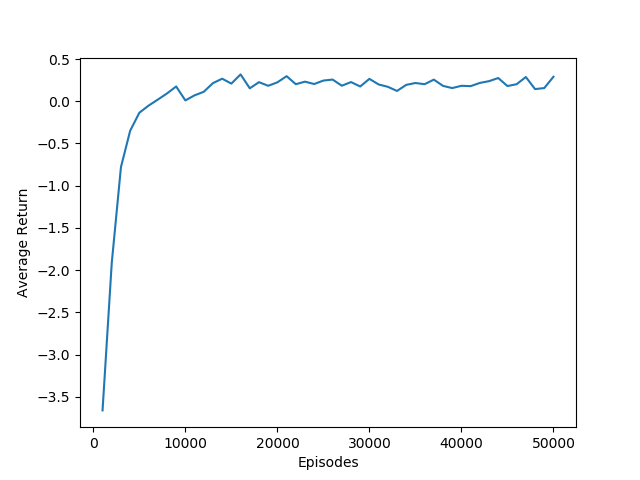
\includegraphics[width=\linewidth]{bonus_a_training.png}
		\caption{Average return versus episodes elapsed during training of policy with the opponent going first half the time.}
		\label{bonus training curve}
\end{figure}

\begin{figure}
		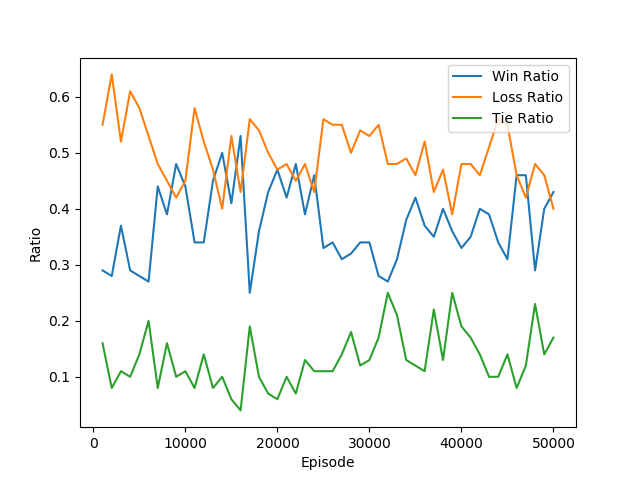
\includegraphics[width=\linewidth]{bonus_a_win_rate_second.png}
		\caption{Win, loss, and tie ratios over training for 100 games for the opponent making the first move.}
		\label{opponent first}
\end{figure}

\begin{figure}
		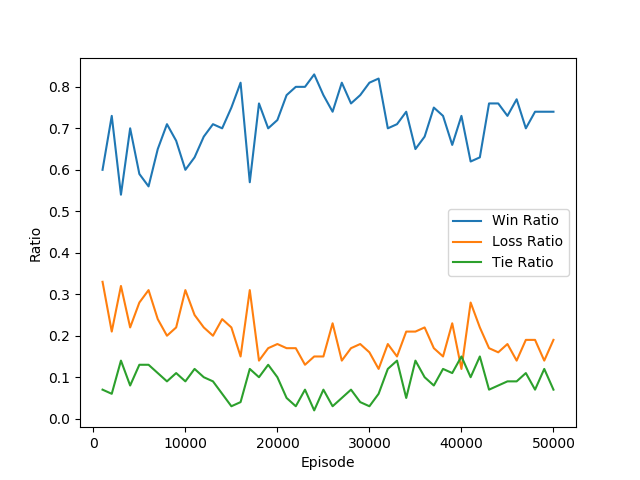
\includegraphics[width=\linewidth]{bonus_a_winrate_first.png}
		\caption{Win, loss, and tie ratios over training for 100 games for the algorithm making the first move.}
		\label{algorithm first}
\end{figure}
\end{problem}

\begin{listing}
		\caption{Five example games from fully trained policy against a random player.}
		\label{5 games}
		\centering
		\begin{minipage}[t]{0.1\linewidth}
			\begin{verbatim}
o.x
...
...
====
oox
.x.
...
====
oox
.x.
o.x
====
oox
ox.
oxx
====
			\end{verbatim}
		\end{minipage}%
		\begin{minipage}[t]{0.1\linewidth}
			\begin{verbatim}
...
.x.
...
====
..o
.x.
...
====
..o
.x.
o.x
====
oxo
.x.
o.x
====
oxo
.x.
oxx
====
			\end{verbatim}
		\end{minipage}%
		\begin{minipage}[t]{0.1\linewidth}
			\begin{verbatim}
..x
...
...
====
..x
.o.
...
====
.ox
.o.
..x
====
xox
.o.
.ox
====
			\end{verbatim}
		\end{minipage}%
		\begin{minipage}[t]{0.1\linewidth}
			\begin{verbatim}
...
..x
...
====
..o
..x
...
====
..o
.xx
o..
====
oxo
.xx
o..
====
oxo
oxx
o.x
====		
			\end{verbatim}
		\end{minipage}%
		\begin{minipage}[t]{0.1\linewidth}
			\begin{verbatim}
.ox
...
...
====
.ox
o..
..x
====
xox
o..
.ox
====
xox
ox.
.ox
====
			\end{verbatim}
		\end{minipage}%
	\end{listing}
\clearpage

%----------------------------------------------------------------------------------------
%	PART 2
%----------------------------------------------------------------------------------------
\FloatBarrier
\begin{problem}
Next, the algorithm was trained by playing \textit{itself}; this means that the opponent progressively gets better throughout training. The training curve is seen in Figure \ref{b training curve}. As expected, the graph is not as interpretable as before since the opponent is no longer random.\\

Figure \ref{b winrate first} and Figure \ref{b winrate second} show the win, loss, and tie ratios for the algorithm making the first and second moves, respectively. Once again, as explained earlier, when the algorithm makes the second move it is less likely to win. This is a natural consequence of the fact that it is an advantage to make the first move in a game of tic-tac-toe.\\

Listing \ref{b 5 games against itself} shows 5 example games where the algorithm plays against itself, and listing \ref{b 5 games against random} shows 5 games against a random opponent.

\begin{figure}
		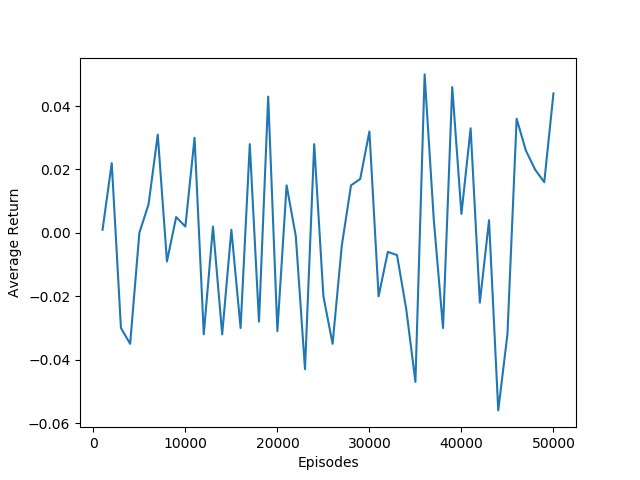
\includegraphics[width=\linewidth]{bonus_b_training.png}
		\caption{Training curve against itself.}
		\label{b training curve}
\end{figure}

\begin{figure}
		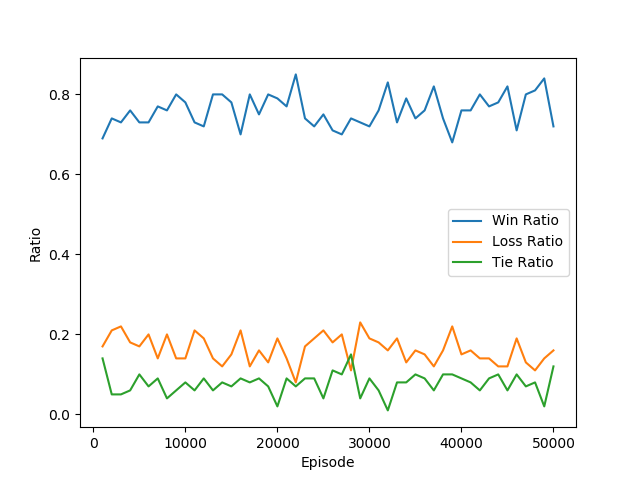
\includegraphics[width=\linewidth]{bonus_b_winrate_first.png}
		\caption{Win, loss, and tie ratios over training for 100 games against random for the algorithm making the first move.}
		\label{b winrate first}
\end{figure}

\begin{figure}
		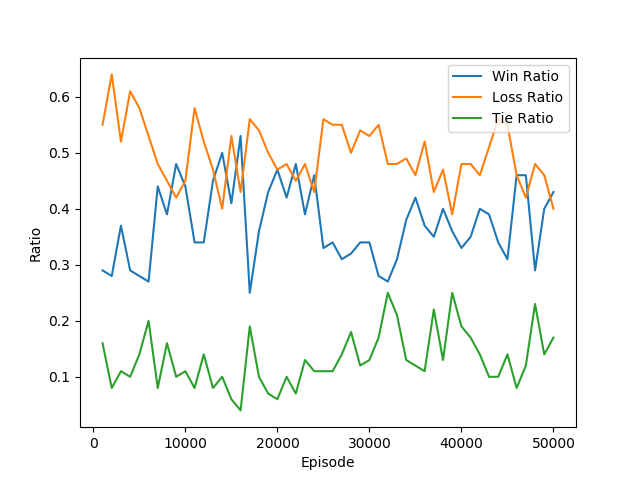
\includegraphics[width=\linewidth]{bonus_a_win_rate_second.png}
		\caption{Win, loss, and tie ratios over training for 100 games against random for the algorithm making the second move.}
		\label{b winrate second}
\end{figure}


\begin{listing}
		\caption{Five example games from fully trained policy against itself.}
		\label{b 5 games against itself}
		\centering
		\begin{minipage}[t]{0.1\linewidth}
			\begin{verbatim}
.x.
====
.xo
====
.xo
..x
====
.xo
.o.
..x
====
.xo
.ox
..x
====
oxo
.ox
..x
====
oxo
.ox
x.x
====
oxo
oox
x.x
====
oxo
oox
xxx
====
			\end{verbatim}
		\end{minipage}%
		\begin{minipage}[t]{0.1\linewidth}
			\begin{verbatim}
.x.
====
..o
.x.
====
.xo
.x.
====
.xo
.x.
..o
====
.xo
.x.
x.o
====
.xo
ox.
x.o
====
xxo
ox.
x.o
====
xxo
ox.
xoo
====
xxo
oxx
xoo
====
			\end{verbatim}
		\end{minipage}%
		\begin{minipage}[t]{0.1\linewidth}
			\begin{verbatim}
..x
====
..x
.o.
====
..x
.o.
..x
====
.ox
.o.
..x
====
xox
.o.
..x
====
xox
.o.
.ox
====
			\end{verbatim}
		\end{minipage}%
		\begin{minipage}[t]{0.1\linewidth}
			\begin{verbatim}
x..
====
x.o
====
x.o
.x.
====
x.o
.o.
.x.
====
xxo
.o.
.x.
====
xxo
.o.
.xo
====
xxo
xo.
.xo
====
xxo
xo.
oxo
====
			\end{verbatim}
		\end{minipage}%
		\begin{minipage}[t]{0.1\linewidth}
			\begin{verbatim}
x..
====
x..
..o
====
x..
.xo
====
x..
.o.
.xo
====
x.x
.o.
.xo
====
xox
.o.
.xo
====
xox
.o.
xxo
====
xox
.oo
xxo
====
xox
xoo
xxo
====
			\end{verbatim}
		\end{minipage}%
	\end{listing}
\clearpage




\begin{listing}
		\caption{Five example games from fully trained policy against random.}
		\label{b 5 games against random}
		\centering
		\begin{minipage}[t]{0.1\linewidth}
			\begin{verbatim}
..x
...
..o
====
..x
ox.
..o
====
..x
ox.
x.o
====
			\end{verbatim}
		\end{minipage}%
		\begin{minipage}[t]{0.1\linewidth}
			\begin{verbatim}
..x
...
.o.
====
..x
.o.
.ox
====
x.x
oo.
.ox
====
x.x
oox
.ox
====
			\end{verbatim}
		\end{minipage}%
		\begin{minipage}[t]{0.1\linewidth}
			\begin{verbatim}
..x
...
.o.
====
..x
.x.
oo.
====
o.x
.x.
oox
====
oxx
.xo
oox
====
oxx
xxo
oox
====
			\end{verbatim}
		\end{minipage}%
		\begin{minipage}[t]{0.1\linewidth}
			\begin{verbatim}
...
x..
...
====
...
x..
..o
====
o.x
x..
..o
====
o.x
xx.
o.o
====
oxx
xxo
o.o
====
oxx
xxo
oxo
====
			\end{verbatim}
		\end{minipage}%
		\begin{minipage}[t]{0.1\linewidth}
			\begin{verbatim}
..x
...
..o
====
..x
ox.
..o
====
x.x
ox.
.oo
====
x.x
ox.
xoo
====
			\end{verbatim}
		\end{minipage}%
	\end{listing}
\clearpage

\end{problem}
\clearpage
%----------------------------------------------------------------------------------------

\end{document}